\documentclass[aspectratio=1610]{beamer}
\setbeamersize{text margin left=7mm,text margin right=5mm}
\usefonttheme[onlymath]{serif}
\usetheme{default}
\usefonttheme{professionalfonts}
%\setbeamertemplate{navigation symbols}{} 
\beamertemplatenavigationsymbolsempty
\addtobeamertemplate{navigation symbols}{}{
    \usebeamerfont{footline}
    \usebeamercolor[fg]{footline}
    %\hspace{1em}
    \footnotesize\insertframenumber\,%/\inserttotalframenumber
}

\usepackage[round]{natbib}
%\bibliographystyle{plainnatnourl} 

% cSpell:disable
\definecolor{rcomment}{rgb}{0.3, 0.3, 0.3}  % darkgrey
\definecolor{rred}{rgb}{0.7,0.2,0.2}        % red
\definecolor{rblue}{rgb}{0.2,0.2,0.7}       % blue (blended blue of beamer)
\definecolor{rpurple}{rgb}{0.45, 0.0, 0.9}  % violett
\definecolor{rpink}{rgb}{0.8, 0.0, 0.4}     % pink
\definecolor{rgreen}{rgb}{0.1, 0.5, 0.1}    % darkgreen
\definecolor{rorange}{rgb}{0.8, 0.4,0}      % orange
\definecolor{rblack}{rgb}{0, 0, 0}          % black
\definecolor{deeptuerkis}{rgb}{0, 0.5, 0.5} % Türkis
\definecolor{darkgreen}{rgb}{0,0.5,0}
\definecolor{blendedblue}{rgb}{0.2,0.2,0.7}
\newcommand{\important}[1]{{\color{green!60!black}#1}}


% \documentclass{beamer}
% \mode<presentation> {
%   \usetheme{Singapore}
%   \setbeamertemplate{navigation symbols}{}
%   \setbeamertemplate{footline}[frame number]
% }

\usepackage[utf8]{inputenc}
\usepackage{caption}
\usepackage{nicefrac}
\usepackage{varwidth}
\usepackage{amsmath}
\usepackage{hyperref}
\usepackage{color}
\usepackage{xcolor}
\usepackage[linesnumbered, ruled, noend]{algorithm2e}
\usepackage{appendixnumberbeamer}
\usepackage{booktabs}
\usepackage{multirow}


\usepackage{natbib}
% \usepackage[backend=bibtex,style=authoryear-comp]{biblatex}
% \bibliography{bibliography}

\usepackage[draft,nomargin,inline]{fixme}  % add final for disabling remarks
\fxsetface{inline}{\itshape}
\fxsetface{env}{\itshape}
%\fxuselayouts{margin}
%\fxuselayouts{inline}
\fxusetheme{color}

\usepackage{tikz}
\usepackage{pgfplots}
\usetikzlibrary{calc, decorations.markings}
\tikzset{vertex/.style={circle, draw=black}}
\tikzset{tr/.style={draw=white, fill=white, sloped}}
\tikzset{del/.style={draw=red, text=red}}
\tikzset{layer/.style={rectangle, draw=black, minimum width=1.5cm, minimum height=0.75cm}}
\tikzset{plus/.style={
  circle, draw=black, minimum width=0.3cm, inner sep=0cm, outer sep=0cm,
  path picture={
    \draw[black] (path picture bounding box.south) -- (path picture bounding box.north)
                 (path picture bounding box.west) -- (path picture bounding box.east);
  }
}}
\tikzset{buswidth/.style={decoration={
  markings,
  mark=at position 0.5 with {\node[font=\footnotesize] {/};\node[below=3pt] {\tiny #1};}
}, postaction={decorate}}}

\pgfplotsset{compat=1.18}


\newcommand{\tmax}{\ensuremath{t^\mathrm{max}}}
\newcommand{\plim}{\ensuremath{p^\mathrm{lim}}}
\newcommand{\ILP}{\ensuremath{\mathrm{ILP}}}
\newcommand{\ppath}{\ensuremath{p^\mathrm{path}}}
\newcommand{\Tavail}{T^\mathrm{avail}}
\newcommand{\Irej}{I^\mathrm{rej}}
\newcommand{\Greedy}{\textsc{Greedy}}
\newcommand{\Markov}{\textsc{Markov}}

\pgfplotsset{compat=newest}
\usepgfplotslibrary{statistics}

\usepackage{tikz}
\usetikzlibrary{arrows,automata}
\usetikzlibrary{datavisualization}
\usetikzlibrary{positioning}
\usetikzlibrary{calc}
\usetikzlibrary{patterns}
\usetikzlibrary{matrix}
\usetikzlibrary{decorations.pathreplacing}
\usetikzlibrary{shapes.geometric, arrows, arrows.meta}

\tikzstyle{vertex} = [circle, draw=black, fill=black, minimum width=0.15cm, inner sep=0cm, text centered]
\tikzstyle{arc} = [thick,->,>=stealth]
\tikzstyle{emphvertex} = [circle, draw=red, fill=red, minimum width=0.15cm, inner sep=0cm, text centered]
\tikzstyle{empharc} = [thick,->,>=stealth, draw=red]
\tikzstyle{vertex-green} = [circle, draw=ForestGreen, fill=ForestGreen, minimum width=0.15cm, inner sep=0cm, text centered]
\tikzstyle{arc-green} = [very thick,->,>=stealth, draw=ForestGreen] %thick, very thick, ultra thick
\tikzstyle{bgvertex} = [circle, draw=black!40, fill=black!40, minimum width=0.15cm, inner sep=0cm, text centered]
\tikzstyle{bgarc} = [draw=black!40,thick,->,>=stealth]
\tikzstyle{move} = [thick, ->, -Implies, double,double distance=0.7mm]
\tikzstyle{cyclearc} = [thick,->,>=stealth,draw=red]
\tikzstyle{gets} = [thick, ->, -{Implies[length=5mm, width=3mm]}, double, double distance=1mm]

\usepackage{rotating}
\usepackage{subcaption}
\usepackage{cancel}

\newcommand\hcancel[2][black]{\setbox0=\hbox{$#2$}%
\rlap{\raisebox{.45\ht0}{\textcolor{#1}{\rule{\wd0}{1pt}}}}#2} 


% CHEATING DASH FROM https://tex.stackexchange.com/a/133357/128068
\tikzset{
	cheating dash/.code args={on #1 off #2}{
		% Use csname so catcode of @ doesn't have do be changed.
		\csname tikz@addoption\endcsname{%
			\pgfgetpath\currentpath%
			\pgfprocessround{\currentpath}{\currentpath}%
			\csname pgf@decorate@parsesoftpath\endcsname{\currentpath}{\currentpath}%
			\pgfmathparse{\csname pgf@decorate@totalpathlength\endcsname-#1}\let\rest=\pgfmathresult%
			\pgfmathparse{#1+#2}\let\onoff=\pgfmathresult%
			\pgfmathparse{max(floor(\rest/\onoff), 1)}\let\nfullonoff=\pgfmathresult%
			\pgfmathparse{max((\rest-\onoff*\nfullonoff)/\nfullonoff+#2, #2)}\let\offexpand=\pgfmathresult%
			\pgfsetdash{{#1}{\offexpand}}{0pt}}%
	}
}


\usepackage[normalem]{ulem} % for strikethrough text
\newcommand\soutred{\bgroup\markoverwith{\textcolor{red}{\rule[0.5ex]{2pt}{0.4pt}}}\ULon} % for crossing out text in red


%******************************
%rest of frame
\usepackage{zref-savepos}

\newcounter{restofframe}
\newsavebox{\restofframebox}
\newlength{\mylowermargin}
\setlength{\mylowermargin}{2pt}

\newenvironment{restofframe}{%
	\par\centering
	\stepcounter{restofframe}%
	\zsavepos{restofframe-\arabic{restofframe}-begin}%
	\begin{lrbox}{\restofframebox}%
	}{%
\end{lrbox}%
\setkeys{Gin}{keepaspectratio}%
\raisebox{\dimexpr-\height+\ht\strutbox\relax}[0pt][0pt]{%
	\resizebox*{!}{\dimexpr\zposy{restofframe-\arabic{restofframe}-begin}sp-\zposy{restofframe-\arabic{restofframe}-end}sp-\mylowermargin\relax}%
	{\usebox{\restofframebox}}%
}%
\vskip0pt plus 1filll\relax
\mbox{\zsavepos{restofframe-\arabic{restofframe}-end}}%
\par 
}

\let\oldfootnotesize\footnotesize
\renewcommand*{\footnotesize}{\oldfootnotesize\fontsize{6}{4}\selectfont}

% reset footnote counter for each frame
\AtBeginEnvironment{frame}{\setcounter{footnote}{0}}

% command for bold blue text
%\DeclareTextFontCommand{\structure}{\color{TuWienBlue}\bfseries}



% \renewcommand{\thefootnote}{\fnsymbol{footnote}}
% cSpell:enable

\title{An Exact Hybrid Solution Approach for a Prize-Collecting Single Machine Scheduling Problem}

\author{Günther R.\ Raidl}
\date{Victoria University of Wellington, NZ\\March 11, 2025}
\titlegraphic{\includegraphics[height=7mm]{graphics/logo-tuwien-informatics.png}\quad
	\includegraphics[height=7mm]{graphics/AClongColor.pdf}}

\institute[]{\normalsize Algorithms and Complexity Group, TU Wien, Austria,\\
    \texttt{raidl@ac.tuwien.ac.at}\\[1ex]
}

\logo{\includegraphics[height=15pt]{graphics/logo.pdf}\vspace{245pt}} % Logo on top right

% cSpell:disable
\definecolor{rred}{rgb}{0.7,0.2,0.2}         % red
\newcommand{\hl}[1]{\textcolor{rred}{#1}}    % highlight

\definecolor{rgreen}{rgb}{0.216,0.784,0.216} % green
\definecolor{rblue}{rgb}{0.216,0.443,0.784}  % blue
\definecolor{rorange}{rgb}{1.0,0.4,0.0}      % orange

\definecolor{orange}{RGB}{255,100,66}
\definecolor{seaborn0}{HTML}{1f77b4}
\definecolor{seaborn1}{HTML}{ff7f0e}
\definecolor{seaborn2}{HTML}{2ca02c}
\definecolor{seaborn3}{HTML}{d62728}
\definecolor{seaborn4}{HTML}{9467bd}
\definecolor{seaborn5}{HTML}{8c564b}
\definecolor{seaborn6}{HTML}{e377c2}
\definecolor{seaborn7}{HTML}{7f7f7f}
\definecolor{seaborn8}{HTML}{bcbd22}
\definecolor{seaborn9}{HTML}{17becf}

\newbool{printlegend}

\newcommand{\cumuldistr}[7]{ % Arguments: source directory, data series, width, height, x label, y label, title
  \begin{tikzpicture}
    \begin{semilogxaxis}[%
          width={#3},
          height={#4},
          title style={align=center},
          title={\large #7},
          xlabel style={at={(axis description cs:0.5,-0.1)},anchor=north},
          xlabel=#5,
          ylabel style={align=center},
          ylabel=#6,
          every axis plot post/.append style={mark=none},
          every axis plot/.append style={thick},
          legend entries={GNN,Random,Sorted,Hooker},
          \ifbool{printlegend}{
            legend columns=1,
            legend pos=south east,
          }{
            legend to name=legend:cumuldistr-#1-#2,
            legend columns=-1,
          }
          ]
      \addplot+[seaborn0, solid]  table [x=#2, y=no_instances, col sep=comma, mark=none] {#1/pgdeletion_#2.csv};
      \addplot+[seaborn1, dashed] table [x=#2, y=no_instances, col sep=comma, mark=none] {#1/deletion_#2.csv};
      \addplot+[seaborn2, dashed] table [x=#2, y=no_instances, col sep=comma, mark=none] {#1/sdeletion_#2.csv};
      \addplot+[seaborn3, dashed] table [x=#2, y=no_instances, col sep=comma, mark=none] {#1/hdeletion_#2.csv};
    \end{semilogxaxis}
  \end{tikzpicture}
}
% cSpell:enable
\renewcommand{\footnotesize}{\scriptsize}

\begin{document}{}


\part{Main}

\begin{frame}
  \titlepage
\end{frame} 



\begin{frame}
	For details see:

	\bigskip
	\emph{J.~Varga, G.~Raidl, E.~Karlsson, E.~Rönnberg, F.~Lindsten, T.~Rodemann:\\ Speeding up Logic-Based Benders Decomposition by Strengthening Cuts with Graph Neural Networks,\\ Machine Learning, Optimization, and Data Science (LOD) 2023, Springer LNCS 14505, pp.~24--38.}
\end{frame}





\begin{frame}
	\frametitle{Single-Machine Scheduling Problem \citep{2020_horn-et-al_article}}
	\begin{minipage}{0.5\textwidth}
	\begin{itemize}
		\item \important{Single machine}
		\item \important{Tasks} $I=\{1,\ldots,n\}$
		\item \important{Multiple time windows} $W_i$ for each task $i\in I$
		\item \important{Setup times} $s_{i,j}$ between tasks $i,j\in I$
		\item \important{Prize} $q_i$ for each task
		\item \structure{Objective:} Maximize \important{total prize} of tasks scheduled without overlap
	\end{itemize}
	\vspace{1em}
	% \uncover<2->{
	% 	\begin{itemize}
	% 	\item \important{MP:} Select \important{task time window pairs} (TTWP)
	% 	\item \important{SP:} Feasible schedule?
	% 	\item \important{Feasibility cut:} $\widehat{=}$ set of TTWPs
	% 	\item \important{Cut-strengthening:} reduce set
	% 	\end{itemize}
	% }
	\end{minipage}%
	\begin{minipage}{0.5\textwidth}
	\scalebox{0.3}{
		\begin{tikzpicture}
		\node at (2,0) {\includegraphics[height=4cm]{graphics/machine.pdf}};
		\node[rectangle,fill=black!70,minimum width=15cm,minimum height=2cm] at (13.5,0) {};

		\draw[very thick, draw=black] (6,1.5) to (6,-10.5);
		\draw[very thick, draw=black] (21,1.5) to (21,-10.5);

		\node[rectangle,fill=black!40,minimum width=2cm,minimum height=2cm] at (1,-4) {};
		%\only<3,4>{\node[rectangle,fill=rgreen,minimum width=4cm,minimum height=2cm] at (9,-4) {};}
		\node[rectangle,draw=black,minimum width=4cm,minimum height=2cm] at (9,-4) {};
		\node[rectangle,draw=black,minimum width=3cm,minimum height=2cm] at (16.5,-4) {};

		\node[rectangle,fill=black!40,minimum width=4cm,minimum height=2cm] at (2,-7) {};
		%\only<3,4>{\node[rectangle,fill=rgreen,minimum width=6cm,minimum height=2cm] at (9,-7) {};}
		\node[rectangle,draw=black,minimum width=6cm,minimum height=2cm] at (9,-7) {};
		\node[rectangle,draw=black,minimum width=5cm,minimum height=2cm] at (18.5,-7) {};

		\node[rectangle,fill=black!40,minimum width=3cm,minimum height=2cm] at (1.5,-10) {};
		%\only<3>{\node[rectangle,fill=rgreen,minimum width=3cm,minimum height=2cm] at (10.5,-10) {};}
		\node[rectangle,draw=black,minimum width=3cm,minimum height=2cm] at (10.5,-10) {};
		\node[rectangle,draw=black,minimum width=3cm,minimum height=2cm] at (16.5,-10) {};
		\end{tikzpicture}
	}
	\end{minipage}

	Appears as subproblem in
	\begin{itemize}
		\item patient scheduling for radio therapy
		\item avionics scheduling
	\end{itemize}
\end{frame}


\begin{frame}{General Solution Approach}
	\begin{itemize}
		\itemsep2ex
		\item We want to solve the problem exactly with \important{Mixed Integer Linear Programming (MILP)}
		\item \important{Partly easy to formulate:}\\
		Decision variables $x_{iw}\in\{0,1\}$ for each task $i$ and each of its time windows $w$, i.e.,\\
		\important{task/time window pair (TTWP) $(i,w)$}
		\begin{align}
			\max                ~ & \sum_{i\in I}\sum_{w\in W_{i}} q_{i}x_{iw} \label{eq:sms_objective_function} \\
			\operatorname{s.t.} ~ & \sum_{w\in W_{i}} x_{iw} \leq 1, & i\in I \label{eq:sms_at_most_one_time_window_per_task} \\
			%~ & \sum_{(i, w) \in X} (1 - x_{iw}) \geq 1, & X \in \mathcal{F} \label{eq:feasibility_cuts} \\
			%~ & \sum_{i\in I}\sum_{w \in W_{i}(t_1,t_2)} p_{i}x_{iw} \leq t_{2} - t_{1}, & (t_{1}, t_{2})\in T \label{eq:sms_segment_relaxation} \\
			~ & x_{iw} \in \{0, 1\}, & i \in I,\ w \in W_{i}.
		\end{align}
		\item<2-> \alert{Missing: The selected TTWPs must allow a feasible solution!} 
		\item<3> Let us assume we know the set $\mathcal{F}$ of \important{all subsets $X$ of TTWPs that do \textbf{not} allow a feasible schedule}, then
		\alert{\begin{equation}
		\sum_{(i, w) \in B} x_{iw} \le |X|-1, \qquad B \in \mathcal{F}
		\end{equation}}
	\end{itemize}
\end{frame}



\begin{frame}
	\frametitle{Single-Machine Scheduling Problem \citep{2020_horn-et-al_article}}
	\begin{minipage}{0.5\textwidth}
	\begin{itemize}
		\item \important{Single machine}
		\item \important{Tasks} with \important{multiple time windows}
		\item \important{Setup times} between tasks
		\item \important{Prize} for each task
		\item Objective: Maximize \important{total prize} of scheduled tasks
	\end{itemize}
	\vspace{1em}
	\only<1>{
		\alert{The three green TTWPs do not allow\\
		a feasible schedule!\\
		$\rightarrow x_{1,1} + x_{2,1} + x_{3,1} \le 2$}
	}
	\only<2>{
		But $x_{1,1} + x_{2,1} + x_{3,1}=3$ is feasible.
	}
	% \only<2->{
	% 	\begin{itemize}
	% 	\item \important{MP:} Select \important{task time window pairs} (TTWP)
	% 	\item \important{SP:} Feasible schedule?
	% 	\item \important{Feasibility cut:} $\widehat{=}$ set of TTWPs
	% 	\item \important{Cut-strengthening:} reduce set
	% 	\end{itemize}
	% }
	\end{minipage}%
	\begin{minipage}{0.5\textwidth}
	\scalebox{0.3}{
		\begin{tikzpicture}
		\node at (2,0) {\includegraphics[height=4cm]{graphics/machine.pdf}};
		\node[rectangle,fill=black!70,minimum width=15cm,minimum height=2cm] at (13.5,0) {};

		\draw[very thick, draw=black] (6,1.5) to (6,-10.5);
		\draw[very thick, draw=black] (21,1.5) to (21,-10.5);

		\node[rectangle,fill=black!40,minimum width=2cm,minimum height=2cm] at (1,-4) {};
		\only<1,2>{\node[rectangle,fill=rgreen,minimum width=4cm,minimum height=2cm] at (9,-4) {};}
		\node[rectangle,draw=black,minimum width=4cm,minimum height=2cm] at (9,-4) {};
		\node[rectangle,draw=black,minimum width=3cm,minimum height=2cm] at (16.5,-4) {};

		\node[rectangle,fill=black!40,minimum width=4cm,minimum height=2cm] at (2,-7) {};
		\only<1,2>{\node[rectangle,fill=rgreen,minimum width=6cm,minimum height=2cm] at (9,-7) {};}
		\node[rectangle,draw=black,minimum width=6cm,minimum height=2cm] at (9,-7) {};
		\node[rectangle,draw=black,minimum width=5cm,minimum height=2cm] at (18.5,-7) {};

		\node[rectangle,fill=black!40,minimum width=3cm,minimum height=2cm] at (1.5,-10) {};
		\only<1>{\node[rectangle,fill=rgreen,minimum width=3cm,minimum height=2cm] at (10.5,-10) {};}
		\node[rectangle,draw=black,minimum width=3cm,minimum height=2cm] at (10.5,-10) {};
		\only<2>{\node[rectangle,fill=rgreen,minimum width=3cm,minimum height=2cm] at (16.5,-10) {};}
		\node[rectangle,draw=black,minimum width=3cm,minimum height=2cm] at (16.5,-10) {};
		\end{tikzpicture}
	}
	\end{minipage}
\end{frame}



\begin{frame}
	\frametitle{Benders Decomposition}
	\begin{centering}
		\includegraphics[width=\textwidth]{graphics/lbbd1}

	\end{centering}
\end{frame}



% \begin{frame}
% 	\frametitle{Single-Machine Scheduling Problem \citep{2020_horn-et-al_article}}
% 	\begin{minipage}{0.5\textwidth}
% 	\begin{itemize}
% 		\item \important{Single machine}
% 		\item \important{Tasks} with \important{multiple time windows}
% 		\item \important{Setup times} between tasks
% 		\item \important{Prize} for each task
% 		\item Objective: Maximize \important{total prize} of scheduled tasks
% 	\end{itemize}
% 	\vspace{1em}
% 	\only<1>{
% 		\alert{The three green TTWPs do not allow\\
% 		a feasible schedule!\\
% 		$\rightarrow x_{1,1} + x_{2,1} + x_{3,1} \le 2$}
% 	}
% 	\only<2->{
% 		\begin{itemize}
% 		\item \important{MP:} Select \important{task time window pairs} (TTWP)
% 		\item \important{SP:} Feasible schedule?
% 		\item \important{Feasibility cut:} $\widehat{=}$ set of TTWPs
% 		\item \important{Cut-strengthening:} reduce set
% 		\end{itemize}
% 	}
% 	\end{minipage}%
% 	\begin{minipage}{0.5\textwidth}
% 	\scalebox{0.3}{
% 		\begin{tikzpicture}
% 		\node at (2,0) {\includegraphics[height=4cm]{graphics/machine.pdf}};
% 		\node[rectangle,fill=black!70,minimum width=15cm,minimum height=2cm] at (13.5,0) {};

% 		\draw[very thick, draw=black] (6,1.5) to (6,-10.5);
% 		\draw[very thick, draw=black] (21,1.5) to (21,-10.5);

% 		\node[rectangle,fill=black!40,minimum width=2cm,minimum height=2cm] at (1,-4) {};
% 		\only<1,2>{\node[rectangle,fill=rgreen,minimum width=4cm,minimum height=2cm] at (9,-4) {};}
% 		\node[rectangle,draw=black,minimum width=4cm,minimum height=2cm] at (9,-4) {};
% 		\node[rectangle,draw=black,minimum width=3cm,minimum height=2cm] at (16.5,-4) {};

% 		\node[rectangle,fill=black!40,minimum width=4cm,minimum height=2cm] at (2,-7) {};
% 		\only<1,2>{\node[rectangle,fill=rgreen,minimum width=6cm,minimum height=2cm] at (9,-7) {};}
% 		\node[rectangle,draw=black,minimum width=6cm,minimum height=2cm] at (9,-7) {};
% 		\node[rectangle,draw=black,minimum width=5cm,minimum height=2cm] at (18.5,-7) {};

% 		\node[rectangle,fill=black!40,minimum width=3cm,minimum height=2cm] at (1.5,-10) {};
% 		\only<1>{\node[rectangle,fill=rgreen,minimum width=3cm,minimum height=2cm] at (10.5,-10) {};}
% 		\node[rectangle,draw=black,minimum width=3cm,minimum height=2cm] at (10.5,-10) {};
% 		\node[rectangle,draw=black,minimum width=3cm,minimum height=2cm] at (16.5,-10) {};
% 		\end{tikzpicture}
% 	}
% 	\end{minipage}
% \end{frame}


\begin{frame}{Subproblem to our Scheduling Problem}

\begin{itemize}
	\itemsep2ex
	\item \important{Find a feasible schedule for a given set of TTWPs $X$ or show infeasibility}
	\item<2> Excellent exact solution method for this: \important{constraint programming (CP)}
	\begin{align}
		\text{find}~ & y_i,\forall i\in I(X)   \\
		\mathrm{s.t.} ~ & \textsc{Disjunctive}((y_{i}\mid i\in I(X)), (p_{i} \mid i \in I(X)), \nonumber\\
		  & \hspace*{3.1cm}(s_{ij}\mid i, j \in I(X)), i\not= j) \label{eq:sub_discjunctive}\\
							~ & r_{iw} \leq y_{i} \leq d_{iw} - p_{i} & (i, w) \in X \label{eq:sub_time_window_constraints}\\
		& y_i\ge 0 & i\in I(X)
	\end{align}
	\item<2> Decision variables $y_i$: actual start time of task $i$
	
\end{itemize}
\end{frame}




\begin{frame}{Benders Decomposition}

(\emph{Benders, 1962})

\bigskip
\begin{itemize}
	\itemsep1.5ex
	\item Prominent exact technique for solving large \important{mixed-integer linear programs (MILPs)}
	\item Breaks down MILP into \important{master} and \important{subproblems}
	\item Master problem (MP) considers only subset of variables/constraints
	\item Solving subproblems (SPs):\\
	via duality we obtain \important{Benders feasibility and/or optimality cuts} for MP
	\item Iterative process
	\item<2> \alert{SPs must be linear programs (LPs), only continuous variables allowed}
\end{itemize}
\end{frame}

\begin{frame}{Logic-Based Benders Decomposition}

\emph{J.\ N.\ Hooker and G.\ Ottosson: Logic-based Benders decomposition. Mathematical Programming, 96:33--60, 2003}

\bigskip
\begin{itemize}
	\itemsep1.5ex
	\item Generalization to essentially \important{arbitrary SPs also incl.\ integral variables}
	\item Unfortunately, \alert{no general systematic way of deriving (strong) Benders cuts} exist anymore
	\item Typically, \important{problem-specific cut-strengthening techniques} are applied,\\ exploiting problem structure
\end{itemize}

\bigskip
\structure{Also related:}
\begin{itemize}
	\item Branch and check (\emph{Hooker and Ottosson, 2003})\\
	MP only solved once, SPs when feasible solutions are encountered
	\item \emph{G.~Codato and M.~Fischetti: Combinatorial Benders cuts for mixed-integer linear programming. Operations Research, 54:756--766, 2006} \nocite{2006_codato-fischetti_article}
\end{itemize}

\end{frame}
	



\begin{frame}
	\frametitle{Cut Strengthening in Logic Based Benders Decomposition}
	\begin{centering}
		\includegraphics[width=\textwidth]{graphics/lbbd2}
	\end{centering}

	\bigskip
	Our approach: \important{Learn strengthening procedure}
\end{frame}

\begin{frame}{Cut Strengthening Methods}

\structure{Deletion filter:}
\begin{itemize}
	\item Consider TTWPs iteratively and try to remove each
	\item Accept removal when subproblem remains infeasible
	\item $\rightarrow $ \important{irreducible set of TTWPs / cut}
	\item Order of TTWPs is crucial, but ``best'' order unknown!
\end{itemize}

\bigskip
\structure{MARCO (Liffiton and Malik, 2013):}
\begin{itemize}
	\item Enumerates \important{\emph{all} irreducible sets of TTWPs} systematically
	\item Much more expensive in terms of SPs to check
\end{itemize}

\bigskip 
\citet{karlsson2021strengthening}: Comparison of different cut strengthening procedures

\bigskip
Our approach: based on the faster deletion filter,\\
but for obtaining training data we use MARCO.
\end{frame}


\section{Learning the Strengthening of Cuts}

\begin{frame}
	\frametitle{GNN-Based Cut-Strengthening}
	Learn \important{Graph Neural Network (GNN) based function}
	\begin{equation*}
	f_\Theta(
		\,\overbrace{I}^\text{\hspace{-1cm}instance\hspace{-1cm}}\,,
		\,\underbrace{X}_\text{\hspace{-1cm}TTWPs from MP\hspace{-1cm}}\,,
		\,\overbrace{S}^\text{\hspace{-1cm}selected TTWPs\hspace{-1cm}}\,
	)
	\qquad \longrightarrow \qquad
	\underbrace{(i,w)}_\text{next TTWP to add to $S$} \text{ and }\quad
	\underbrace{\tau}_\text{stop?}
	\end{equation*}

	\bigskip
	\uncover<1->{
	\noindent\important{Given:} problem instance $I$, feasibility cut $X$ \\
	\important{Return:} strengthened feasibility cut
	\begin{enumerate}
		\item Start with $S=[]$
		\item Autoregressively add TTWPs $(i,w)$ until $\tau$
		\item Autoregressively add TTWPs $(i,w)$ until subproblem($S$) is infeasible
		\item Apply deletion filter in reverse order of $S$
	\end{enumerate}
	}
\end{frame}

\begin{frame}
	\frametitle{GNN Architecture\footnote{Inspired by \citet{kool2019attention}}}
	Complete directed graph with nodes $\widehat{=}$ \important{$X$} (TTWPs from MP solution) \\
	\important{Input:} 16 node features $x$, 7 arc features $y$ \\
	\important{Output:} $p$, $\tau$

	% cSpell:disable
	\begin{centering}
	\scalebox{0.7}{
		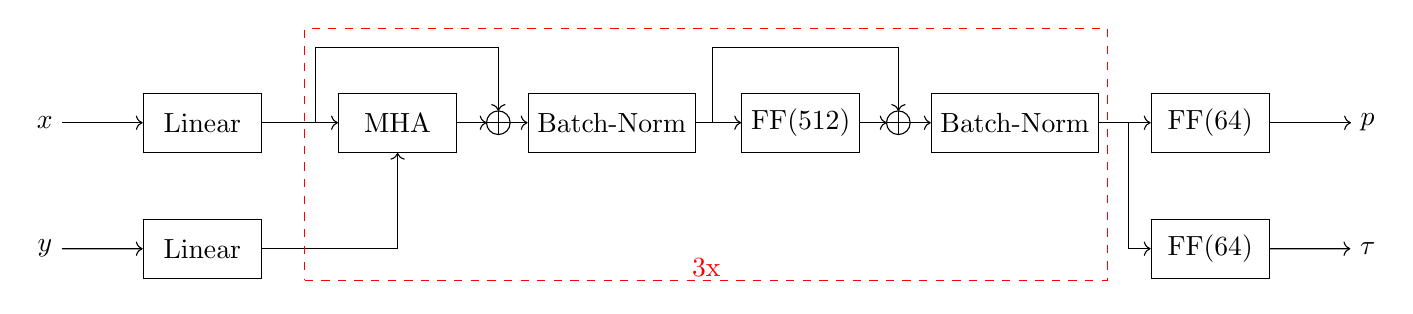
\begin{tikzpicture}[scale=0.8]
		\node at (0,0) (x) {$x$};
		\node[layer] at (2.5,0) (linx) {Linear};
		\node at (0,-2) (y) {$y$};
		\node[layer] at (2.5,-2) (liny) {Linear};
		\node[layer] at (5.6,0) (mha) {MHA};
		\node[plus] at (7.2,0) (skip-mha) {};
		\node[layer] at (9,0) (bn-mha) {Batch-Norm};
		\node[layer] at (12,0) (ff) {FF(512)};
		\node[plus] at (13.55,0) (skip-ff) {};
		\node[layer] at (15.4,0) (bn-ff) {Batch-Norm};
		\node[layer] at (18.5,0) (ffp) {FF(64)};
		\node at (21,0) (p) {$p$};
		\node[layer] at (18.5,-2) (fff) {FF(64)};
		\node at (21,-2) (f) {$\tau$};

		\draw[->] (x) -- (linx);
		\draw[->] (linx) -- (mha);
		\draw[->] (y) -- (liny);
		\draw[->] (liny) -| (mha);
		\draw[->] (mha) -- (skip-mha);
		\draw[->] (linx) -| ++(1.8,1.2) -| (skip-mha);
		\draw[->] (skip-mha) -- (bn-mha);
		\draw[->] (bn-mha) -- (ff);
		\draw[->] (ff) -- (skip-ff);
		\draw[->] (bn-mha) -| ++(1.6,1.2) -| (skip-ff);
		\draw[->] (skip-ff) -- (bn-ff);
		\draw[->] (bn-ff) -- (ffp);
		\draw[->] (ffp) -- (p);
		\draw[->] (bn-ff) ++(1.8,0) |- (fff);
		\draw[->] (fff) -- (f);

		\node[rectangle, draw=red, dashed, minimum width=10.2cm, minimum height=3.2cm] at (10.5,-0.5) {};
		\node[text=red] at (10.5, -2.3) {3x};
		\end{tikzpicture}
	}
	\captionof{figure}{Architecture of the GNN.}
	\end{centering}
	% cSpell:enable

	\important{MHA:} Multi-head attention, i.e., transformer-based convolution layer with 8 heads

	\bigskip
	$f_\Theta$ returns TTWP with maximal $p$ and rounded $\tau$
\end{frame}

\begin{frame}
	\frametitle{Training}
	Offline, in supervised fashion using representative problem instances

	\bigskip
	\structure{Collecting training samples:}

	\medskip
	\begin{enumerate}
	\itemsep2ex
	\item \important{Run Logic-based Benders Decomposition}
		\begin{itemize}
		\item enumerate \important{\emph{all} irreducible cuts} via MARCO, add them to the MP
		\item record all SPs and cuts
		\end{itemize}
	\item Determine a minimal subset of \important{\bf strong cuts},\\
		i.e., cuts actually required in MP to get feasible optimal solution
	\item For each subproblem: \important{Rollouts}
		\begin{itemize}
		\item Start with empty set $S$
		\item Successively add TTWPs leading to a strong cut randomly until $S$ $\widehat{=}$ irreducible cut
		\item \important{Each iteration:} add \important{training sample}
		\item \important{Labels:} based on strong cuts
		\end{itemize}
	\end{enumerate}

	\bigskip
	Loss function: binary cross-entropy
\end{frame}




\begin{frame}[fragile]
	\frametitle{Experiments Setup}
	\begin{itemize}
	\item \important{Instances} like in \emph{Horn, Raidl, and Rönnberg (2021)}, $n\in\{10,15,20,25\}$ tasks
	\item \verb|pytorch_geometric|, Gurobi 9.5, CP\,Optimizer 20.1
	\item AMD Ryzen 9 5900X
	\item For each $n$: 300\,000 to 600\,000 training samples from 2.000 to 200\,000 instances
	\item 40 to 300 training epochs
	\vspace{6mm}
	\item Comparison to \important{deletion filter} with different orders:
		\begin{itemize}
		\item Random
		\item Sorted: natural order from instance
		\item \citet{2013_coban-hooker_article}: sorted by decreasing slack
		\end{itemize}
	\end{itemize}
\end{frame}
 
\begin{frame}
	\frametitle{Results: Number of Solved SPs to Reach Optimality}
	\centering
	\cumuldistr{csv/avionics20_inst20}{no_subproblems_performed}{0.8\textwidth}{0.6\textheight}{\# of solved subproblems}{\# of solved\\instances}{\normalsize 20 Tasks}
	\ref{legend:cumuldistr-csv/avionics20_inst20-no_subproblems_performed}

	\bigskip
	Reduction: $\approx 70\%$
\end{frame}

\begin{frame}
	\frametitle{Results: Time to Reach Optimality}
	\centering
	\cumuldistr{csv/avionics20_inst20}{time_spent}{0.8\textwidth}{0.6\textheight}{Time {[s]}}{\# of solved\\instances}{}\hfill
	\ref{legend:cumuldistr-csv/avionics20_inst20-time_spent}

	\bigskip
	Reduction: $\approx 50\%$
\end{frame}

% \begin{frame}
% 	\frametitle{Results: Number of MP Iterations}
% 	\centering
% 	\cumuldistr{csv/avionics20_inst20}{no_benders_iteration}{0.8\textwidth}{0.6\textheight}{Time {[s]}}{\# of LBBD iterations}{}\hfill
% 	\ref{legend:cumuldistr-csv/avionics20_inst20-no_benders_iteration}
% \end{frame}

% \begin{frame}{Results: Bounds over Time}
% 	\centering
% 	\includegraphics[width=10cm]{graphics/results-bounds.png}\hfill
% 	\ref{legend:cumuldistr-csv/avionics20_inst20-no_benders_iteration}
% \end{frame}

% \begin{frame}{Results: Out-of-Distribution Usage of GNNs}
% 	\centering
% 	25 Tasks\\
% 	\includegraphics[width=15cm]{graphics/results-extrapolation.png}
% \end{frame}

\section{Conclusion}

\begin{frame}
	\frametitle{Conclusion}
	\begin{itemize}
	\itemsep1.5ex
	\item Logic Based Benders Decomposition:\\powerful technique for problems with certain structures
	\item Allows combinations of different solving techniques
	\item Cut-strengthening essential for performance
	\item A learning-based approach can lead to stronger cuts and less overall iterations
	\item Logic Based Benders Decomposition also promising in combination with (meta-)heuristics!
	\end{itemize}
\end{frame}




\begin{frame}[allowframebreaks]
	\frametitle{References}
	\footnotesize
	%\nocite{*} 
	% \bibliographystyle{abbrv}
	\bibliographystyle{apalike}
	\bibliography{lit.bib}
\end{frame}



\end{document}

